\chapter{Modeling the Effects of Feedback}
\label{chapter:modeling}

\section{Introduction}

\subsection{Motivation}
The second Aim of this dissertation is to develop a model of the human pilot which includes the effects of concurrent bandwidth feedback.
The model presented here extends Hess' Structural Model of the human pilot.
The Structural Model has been extremely successful in predicting human performance through a variety of system dynamics and can predict how performance changes during a pilot's adaptation to changing dynamics.
Hess has developed adaptive logic for the human pilot in a pursuit task which triggers when the pilot notices that vehicle dynamics have changed, see Figure~\ref{figure:hesspursuit}~\citep{hess_modeling_2009}.
This logic is based off several criteria, which ``must be predicated upon information available to the human [and] the postadapated pilot models must follow the dictates of the crossover model of the human pilot''~\citep{hess_modeling_2009}.
The primary result of the adaptive logic is to increase the resulting crossover frequency of the pilot, effectively making them more responsive, which could be interpreted as more focused on the task.

\begin{figure}[tb]
    \begin{center}
        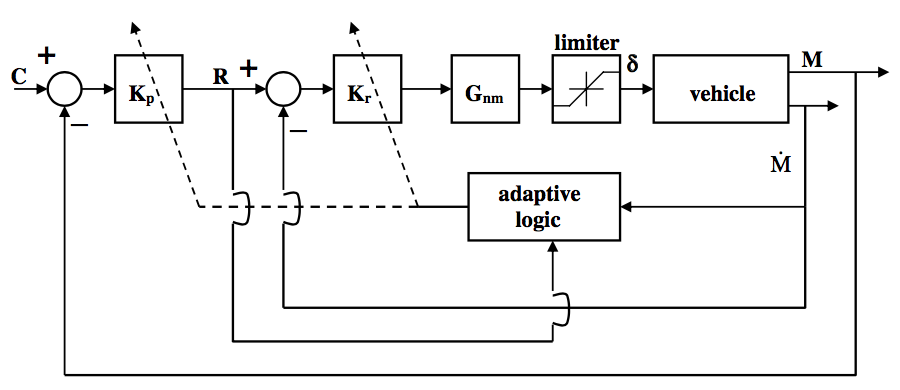
\includegraphics[width=0.8\linewidth]{figures/Modeling/Screen_Shot_2018-08-09_at_4_15_24_PM.png}
        \caption[Hess' model of the adaptive human pilot]{Hess' model of the adaptive human pilot, from~\citet{hess_modeling_2009}.}
        \label{figure:hesspursuit}
    \end{center}
\end{figure}

While this model of the adaptive pilot has been successful in predicting changes in performance for a well-trained subject, it does not consider how a pilot would behave when they are still in the early stages of training.
The modified model presented here includes two major changes to Hess' current model:
\begin{itemize}
    \item The adaptation logic is changed to focus on concurrent bandwidth feedback
    \item The timescale of the adaptation is significantly longer
\end{itemize}

Here, the adaptive logic to triggers when the pilot is receiving concurrent bandwidth feedback, rather than when a change in system dynamics occurs.
This requires the addition of an additional feedback loop onto the Structural Model which triggers when the bandwidth feedback is activated.
This loop is based around the $K_e$ gain, which is the primary way of setting the crossover frequency in the Structural Model.
This change implies that the subjects in our experiments do their primary learning when they are receiving qualitative feedback that their current level of aggressiveness is not sufficient to complete the task.

While there must be a separate loop that adjusts the crossover frequency as learning progresses over the course of several hours, the change in performance we see when subjects use the concurrent bandwidth feedback happens relatively rapidly, within a few minutes.
This is reflected in the delta of performance between subjects in the different groups of our SAFER experiment, even on the first trial, see Figure~\ref{figure:saferdistance}.
This relates to the second required change, the amount of required adaptation time.
Hess' model requires that pilots adapt within a very short time period, on the order of 5 seconds~\citep{weir_model_1966}.
The results of our experiments in the past three chapters suggest relatively long adaptation times, on the order of a few minutes.

\section{Method}

\subsection{The Piloting Task}

\begin{figure}[b]
    \centering
    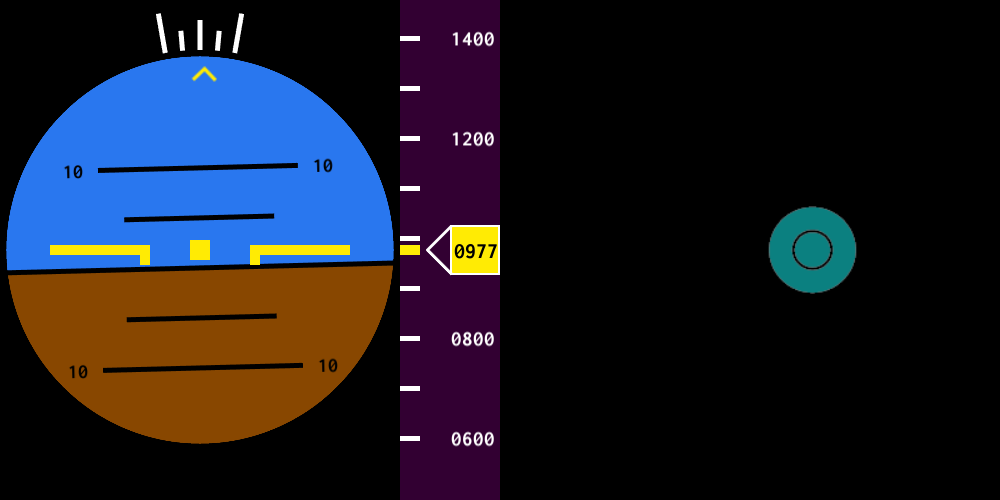
\includegraphics[width=0.8\linewidth]{figures/Aircraft/image1.png}
    \caption[The interface]{The interface that participants were presented with during the experiment, showing the flight task on the right with deviations from nominal in pitch, roll, and altitude, and the secondary, two-choice, task on the right.}
    \label{fig:display}
\end{figure}

Training operators to perform complex manual control tasks is expensive and time consuming, and poorly trained operators can cause catastrophic failures.
The use of concurrent feedback techniques has been shown to improve performance and reduce training times, but had not previously been evaluated for complex, real-world tasks such as flying aircraft.
In the experiment (fully described in Chapter~\ref{chapter:aircraftfeedback}), thirty participants were evenly split into two groups and tasked with flying a simulated Boeing 747 aircraft in three control modes of increasing degrees of freedom and functional complexity.
In order of increasing degrees of freedom and functional complexity, these three control modes were:
\begin{itemize}
    \item[\textbf{P}] Pitch only (low complexity)
    \item[\textbf{PR}] Pitch and Roll (moderate complexity)
    \item[\textbf{PRA}] Pitch, Roll and Altitude (significant complexity)
\end{itemize}

Each participant completed a total of 36 trials: 12 in each of the three control modes.
Each trial had a duration of 82 seconds, and participants self-initiated the trial by activating a trigger on the joystick.
The complete results of this experiment can be seen in Chapter~\ref{chapter:aircraftfeedback}.

% The control group controlled simulated aircraft motion with visual guidance for pitch, roll, and altitude provided by traditional flight instruments.
% The feedback group received additional visual concurrent feedback for each controlled degree of freedom.
The two groups of participants are: control and feedback, and the interface that participants saw during the experiment is available in Figure~\ref{fig:display}.
When the vehicle was well controlled (small errors in the controlled degrees of freedom), the interface was the same for participants in both groups.
Depending on the control mode the the participant was completing, however, participants in the feedback group experienced concurrent bandwidth feedback on various elements of the attitude indicator and altimeter.
This feedback was indicated by changing the element from the default yellow color to a red color when the error deviated outside of a predetermined bandwidth.
For the Pitch only control mode, the display changed from yellow to red when the pitch deviated by greater than three degrees.
% Pitch feedback was provided on the central pitch indicator when the pitch was three or more degrees from zero, roll feedback was provided on the attitude indicator's ``wings'' when the roll was three or more degrees from zero, and attitude feedback was provided on the altimeter text box when the altitude was 30 feet or more off the nominal altitude of 1000 feet.
For both groups, performance measurements were evaluated to determine the effects of the feedback on subject learning rate and maximum skill level.
After the 9th trial, subjects in the feedback group no longer experienced feedback, and the interfaces for the control and feedback groups were the same.
To assess short-term retention of learned skill for the feedback group, the concurrent feedback was removed, and performance was again evaluated.
This was done in order to investigate how well the subjects could retain their performance benefit.

\subsubsection{Experiment Results}
The resulting root-mean-square error for each group of participants by trial is presented in Figure~\ref{fig:prmse}.
Both groups of participants had a relatively high initial root-mean-square error (RMSE) which was reduced through repeated training on the task.
Participants in the feedback group, however, performed significantly better than those in the control group and learned the task much faster.
Additionally, subjects in the feedback group were able to maintain their improved performance when the feedback was removed, and actually show a slight increase in performance when this occurs.

\begin{figure}[tb]
    \centering
    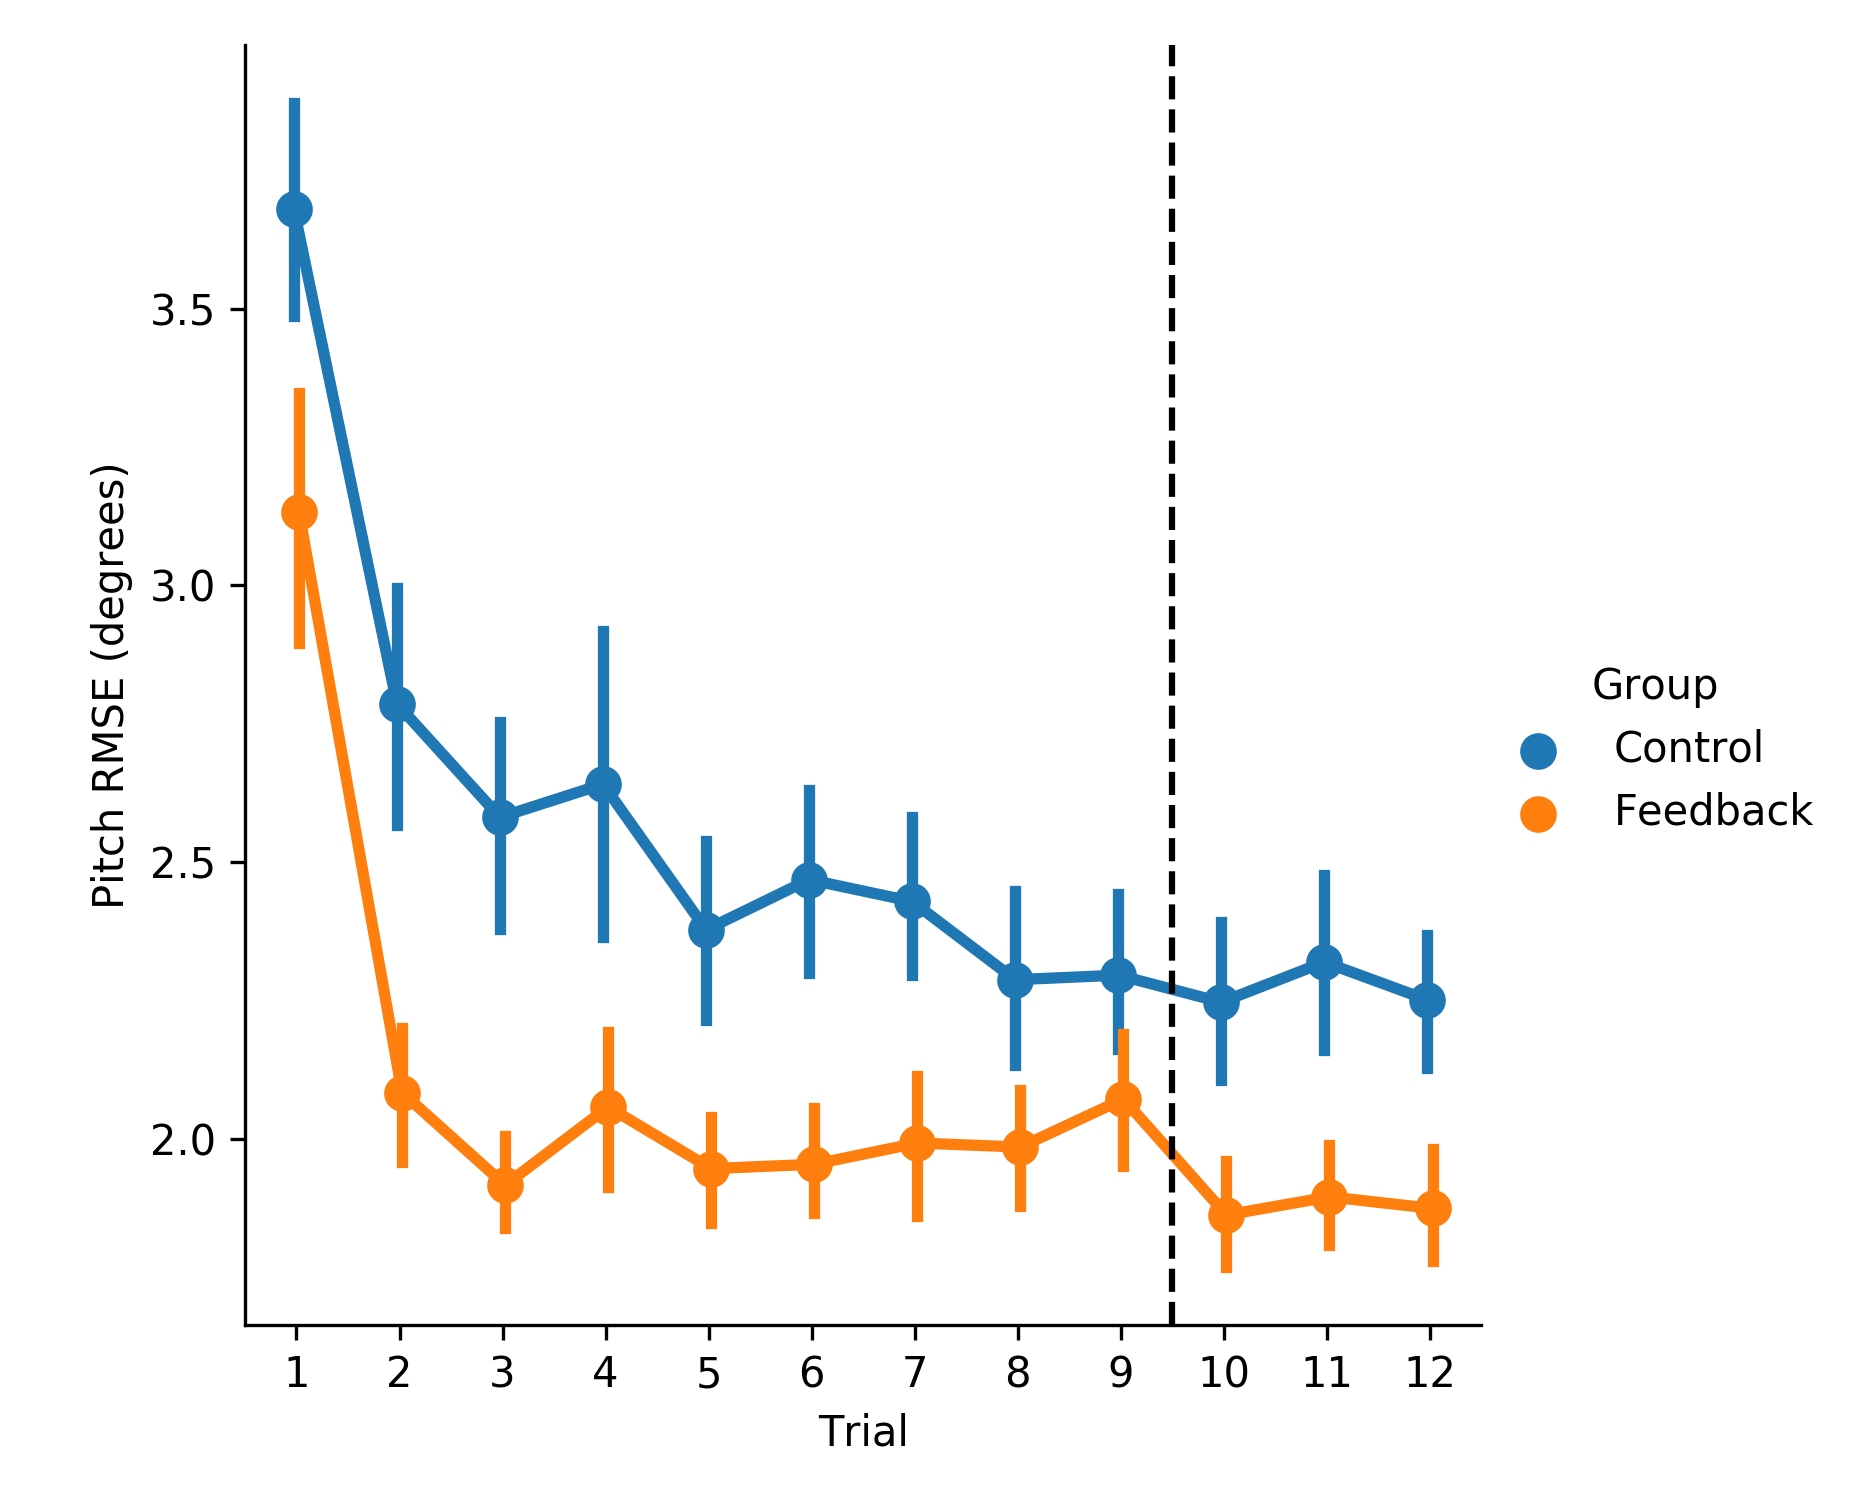
\includegraphics[width=0.8\linewidth]{figures/Modeling/prms_arx.png}
    \caption[Pitch root-mean-square error]{Pitch root-mean-square error. Feedback was removed from subjects in the feedback group after the 9th trial in order to investigate immediate retention.}
    \label{fig:prmse}
\end{figure}

\subsection{Modeling Techniques}
We investigated two techniques for creating models of human pilot in order to better understand the results of the aircraft training study.
Both techniques produce an estimated transfer function of human operator, $Y_p$, which can be combined with the controlled system dynamics, $Y_c$, in order to explore the crossover model characteristics discussed in~\ref{background:pilotmodeling}.
The crossover frequency can be identified using
\begin{align}
    Y_c Y_p = \dfrac{w_c e^{-s \tau_e}}{s}
\end{align}
which provides an indication of how hard the operator is working.
These two techniques are an Autoregressive Model with Exogenous Variables (ARX) technique and the Structural Model.

\subsubsection{Autoregressive Model with Exogenous Variables (ARX)}
Autogregressive (AR) models are commonly used to represent time-varying processes in which an output variable linearly depends on its previous value and a stochastic error term.
When a process also depends on an input variable (often referred to as an exogenous variable), the resulting model is known as an autoregressive model with exogenous variables (ARX).
The structure of an ARX model is given by
% https://www.mathworks.com/help/ident/ref/arx.html
\begin{equation}
    y(t) + a_1 y(t-1) + \ldots + a_{n_a} y(t - n_a) = \\
    b_1 u(t-n_k) + \ldots + b_{n_b} u(t-n_b - n_k+1) + e(t)
\end{equation}
where $y(t)$ is the output variable at time $t$, $n_a$ is the number of poles, $n_b$ is the number of zeros, $n_k$ is the number of input samples which occur between input and output (also known as the dead time or time delay in the system), $y(t-1) \ldots y(t-n_a)$ are the previous outputs on which the current output depends, $u(t-nk) \ldots u(t-n_b - n_k+1)$ are the delayed inputs on which the current output depends, and $e(t)$ is a white-noise error term.

An autoregressive technique to identify a transfer function from an input/output time sequence pair was previously developed in~\citet{hess_modeling_2002}.
Using this technique, called \textit{gettf1}, we identified transfer functions representing pilot models for the data trials from our experiment.
The inputs to this technique are the input and output timeseries and three integers describing the resulting model ($n_a, n_b,$ and $n_k$).
For the results presented in this Chapter, $n_a = n_b = 10$ and $n_k = 0$.
This technique uses an ARX model which is fit using least-squares, and results in a discrete transfer function model estimation of the input/output system.
The script also produces a continuous transfer function using a Tustin approximation.
The result of this process is a transfer function of the pilot with ten poles and zeros describing the human operator's response to the displayed flight dynamics.

\subsubsection{Structural Model}
\begin{figure}[tb]
    \centering
    \begin{subfigure}{\textwidth}
        \centering
        \includegraphics[width=0.8\textwidth]{figures/structural_model/structural_model.pdf}
        \caption[The Structural Model]{The Structural Model, adapted from~\citet{hess_unified_1997}.}
        \label{fig:structuralmodel}
    \end{subfigure}
    \hfill
    \begin{subfigure}{\textwidth}
        \centering
        \includegraphics[width=0.8\textwidth]{figures/structural_model_reduced/structural_model.pdf}
        \caption[The reduced structural model used in this analysis]{The reduced structural model used in this analysis.}
        \label{fig:structuralmodelreduced}
    \end{subfigure}
    \caption[The Structural Model of the Human Pilot]{The Structural Model of the Human Pilot.}
    \label{fig:structuralmodels}
\end{figure}

The complete Structural Model in Figure~\ref{fig:structuralmodel} can be reduced to Figure~\ref{fig:structuralmodelreduced} by setting the following standard parameter values.
\begin{align}
    \nonumber    S_1 = S_2 = S_3 = \enspace \downarrow \\
    \nonumber    K_{\dot{e}} = \epsilon = K_{\dot{m}} = K_{\ddot{m}} = 0
\end{align}
These switches are set to their standard locations for normal error sensing~\citep{hess_unified_1997}.
$K_{\dot{e}}$ is irrelevant as it no longer appears in the loop due to the orientation of the switches, abd $\epsilon$ is set to zero for simplicity.
$K_{\dot{m}}$ and $K_{\ddot{m}}$ are set to zero because the participants did not experience any motion, removing the vestibular feedback loop.

The resulting model can be parameterized by defining $Y_{NM}, Y_{FS},$ and $Y_{PF}$.
$Y_{NM}$ describes the open-loop dynamics of the neuromuscular system driving the joystick, and can be defined
\begin{align}
    Y_{NM} = \frac{\omega^2_{NM}}{s^2 + 2 \zeta_{NM} \omega_{NM} s + \omega^2_{NM}}
\end{align}
where $\omega_{NM}$ and $\zeta_{NM}$ are the undamped natural frequency and damping ratio of the neuromuscular system.
$Y_{FS}$ is set to 1 here, as for a simple joystick it takes the form of a gain which is otherwise absorbed by the other elements in the model.
The proprioceptive feedback block is defined
\begin{align} \label{eq:ypf}
    Y_{PF} = \frac{K}{s+a}
\end{align}
which is is chosen to satisfy $Y_{PF} \propto s Y_c (s)$, and represents the operator's internal model of the system dynamics~\citep{hess_unified_1997}.
Finally, $Y_c$ describes the flight dynamics for the task.
This task dynamics describe a Boeing 747 in Flight Condition 2, and resultant elevator to pitch dynamics take the form~\citep{heffley1972aircraft}:
\begin{align}
    Y_c = \frac{0.5716 (s+0.5535) (s+0.03952)}{(s^2 + 0.006158s + 0.01512) (s^2 + 1.12s + 0.8006)}
\end{align}

\section{Results}

\subsection{ARX}
The original input to the system from the experiment participants $(u)$ can be fed into this resulting transfer function to produce a simulated output $(u_{sim})$.
The resulting output from the pilot models can be compared with the experimental data from which they are generated in order to determine the goodness of fit.
The variance accounted for (VAF) is a commonly used metric to quantify the goodness of the fit between the outputs of the model and the experimental data.
The VAF is calculated by
\begin{equation}
    \mbox{VAF} = \left( 1 - \dfrac{\sum{|u - u_{sim}|^2}} {\sum{u^2}} \right) \times \mbox{100\%}
\end{equation}
where $u$ is the participant's command input to the vehicle's elevators, and $u_{sim}$ is the model's simulated input.
The VAF ranges between 0 (no correlation) and 1 (perfect match).

\begin{figure}[p]
    \centering
    \begin{subfigure}{\textwidth}
        \centering
        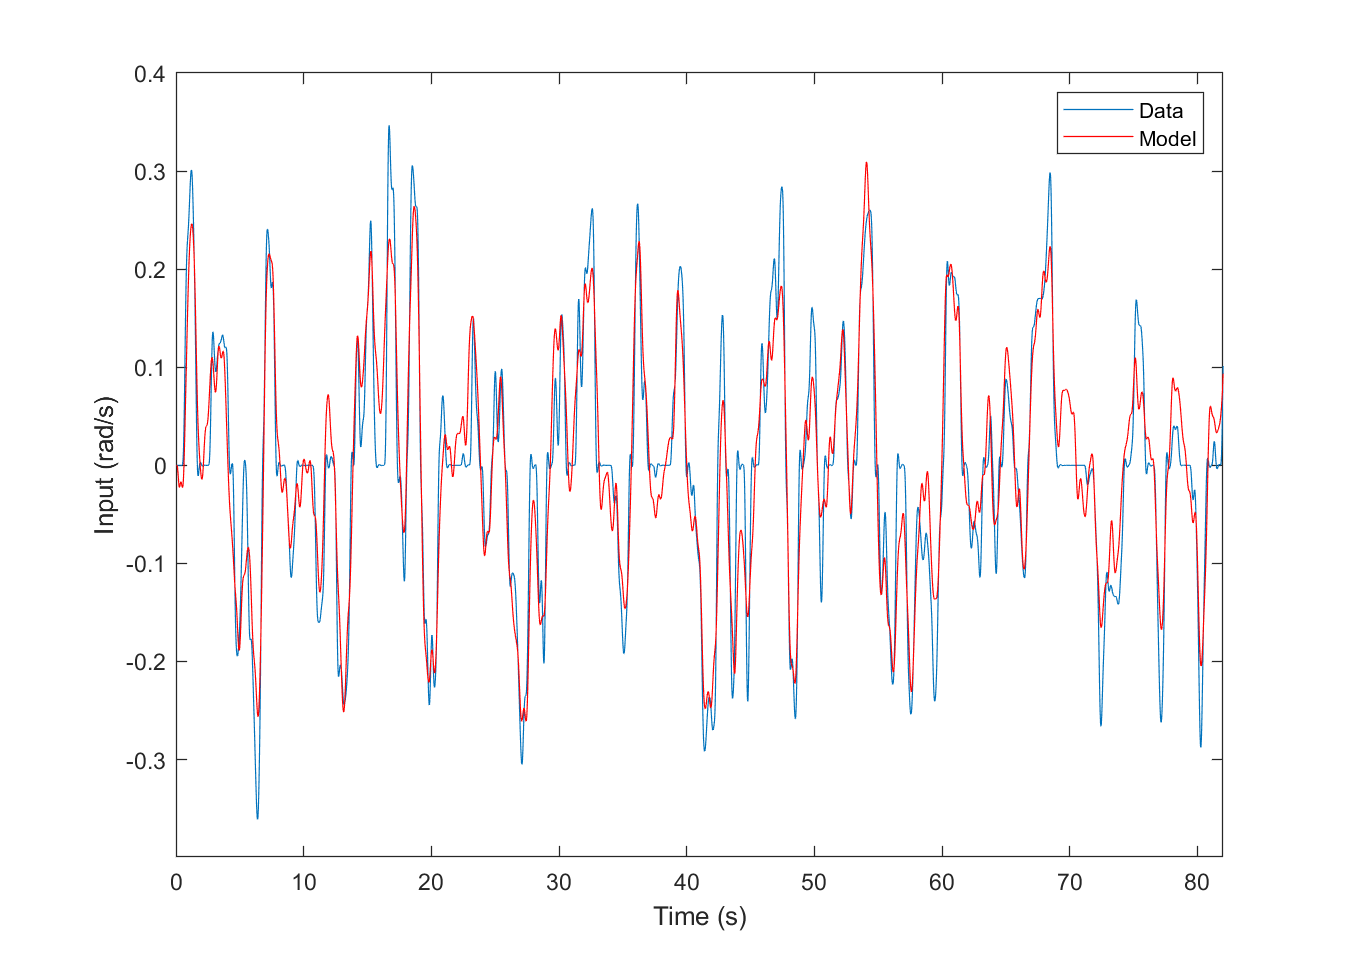
\includegraphics[width=0.9\textwidth]{figures/Modeling/model_output.png}
        \caption[Comparison between estimated transfer function model and experimental data]{Comparison between estimated transfer function model and experimental data.}
        \label{fig:comparison}
    \end{subfigure}
    \hfill
    \begin{subfigure}{\textwidth}
        \centering
        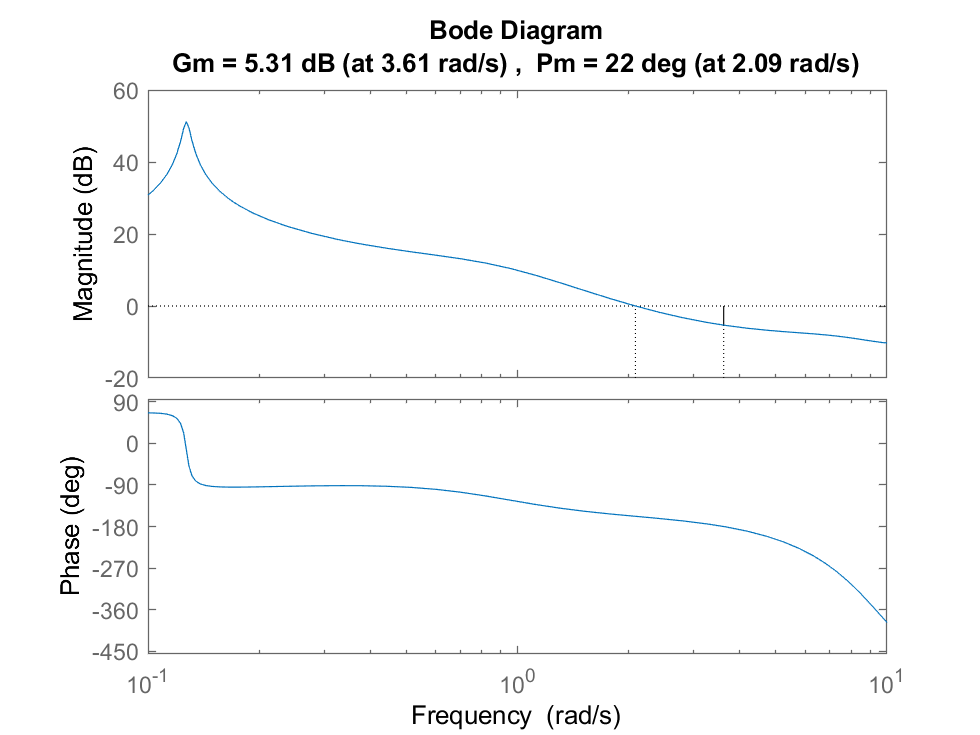
\includegraphics[width=0.9\textwidth]{figures/Modeling/YpYc_204.png}
        \caption[Combined pilot/vehicle open-loop bode diagram]{Combined pilot/vehicle open-loop bode diagram showing the standard crossover model characteristics.}
        \label{fig:bode}
    \end{subfigure}
    \caption[Example results from using the estimated pilot models from \textit{gettf1}]{Example results from using the estimated pilot models from \textit{gettf1}.}
    %    \label{fig:goodnessoffit}
\end{figure}

The VAF of the feedback group's models immediately jumps up after the first trial to an average of $\approx.75$, indicating a good fit.
The control groups VAF increases more slowly, to a value of approximately $\approx.68$.
An increased VAF indicates that the pilot is behaving in a more linear fashion, and these results suggest that the concurrent feedback can immediately assist participants to this end.
The RMSE between the simulated and actual data is similar between groups and trends slightly up during training.
Visual inspection of the experimental and simulated data also shows very good agreement, see Figure~\ref{fig:comparison}.

By combining these pilot models with the system dynamics, the crossover frequency (Figure~\ref{fig:bode}) and gain and phase margins can be found.
The crossover model has long been used as the standard model for human control tasks, where the crossover frequency represents ``how hard'' the pilot is working~\citep{mcruer_dynamic_1957}.
The results of these parameters reflect what was found in the pitch RMSE performance analysis.
Subjects in the feedback group immediately show increased crossover frequency and decreased phase and gain margins.
These results are sustained during retention, and again show an immediate increase/decrease when the feedback is removed.
The crossover frequency identified by the ARX for the pitch only trials is available in Figure~\ref{fig:arx_crossover}.

\begin{figure}[tb]
    \centering
    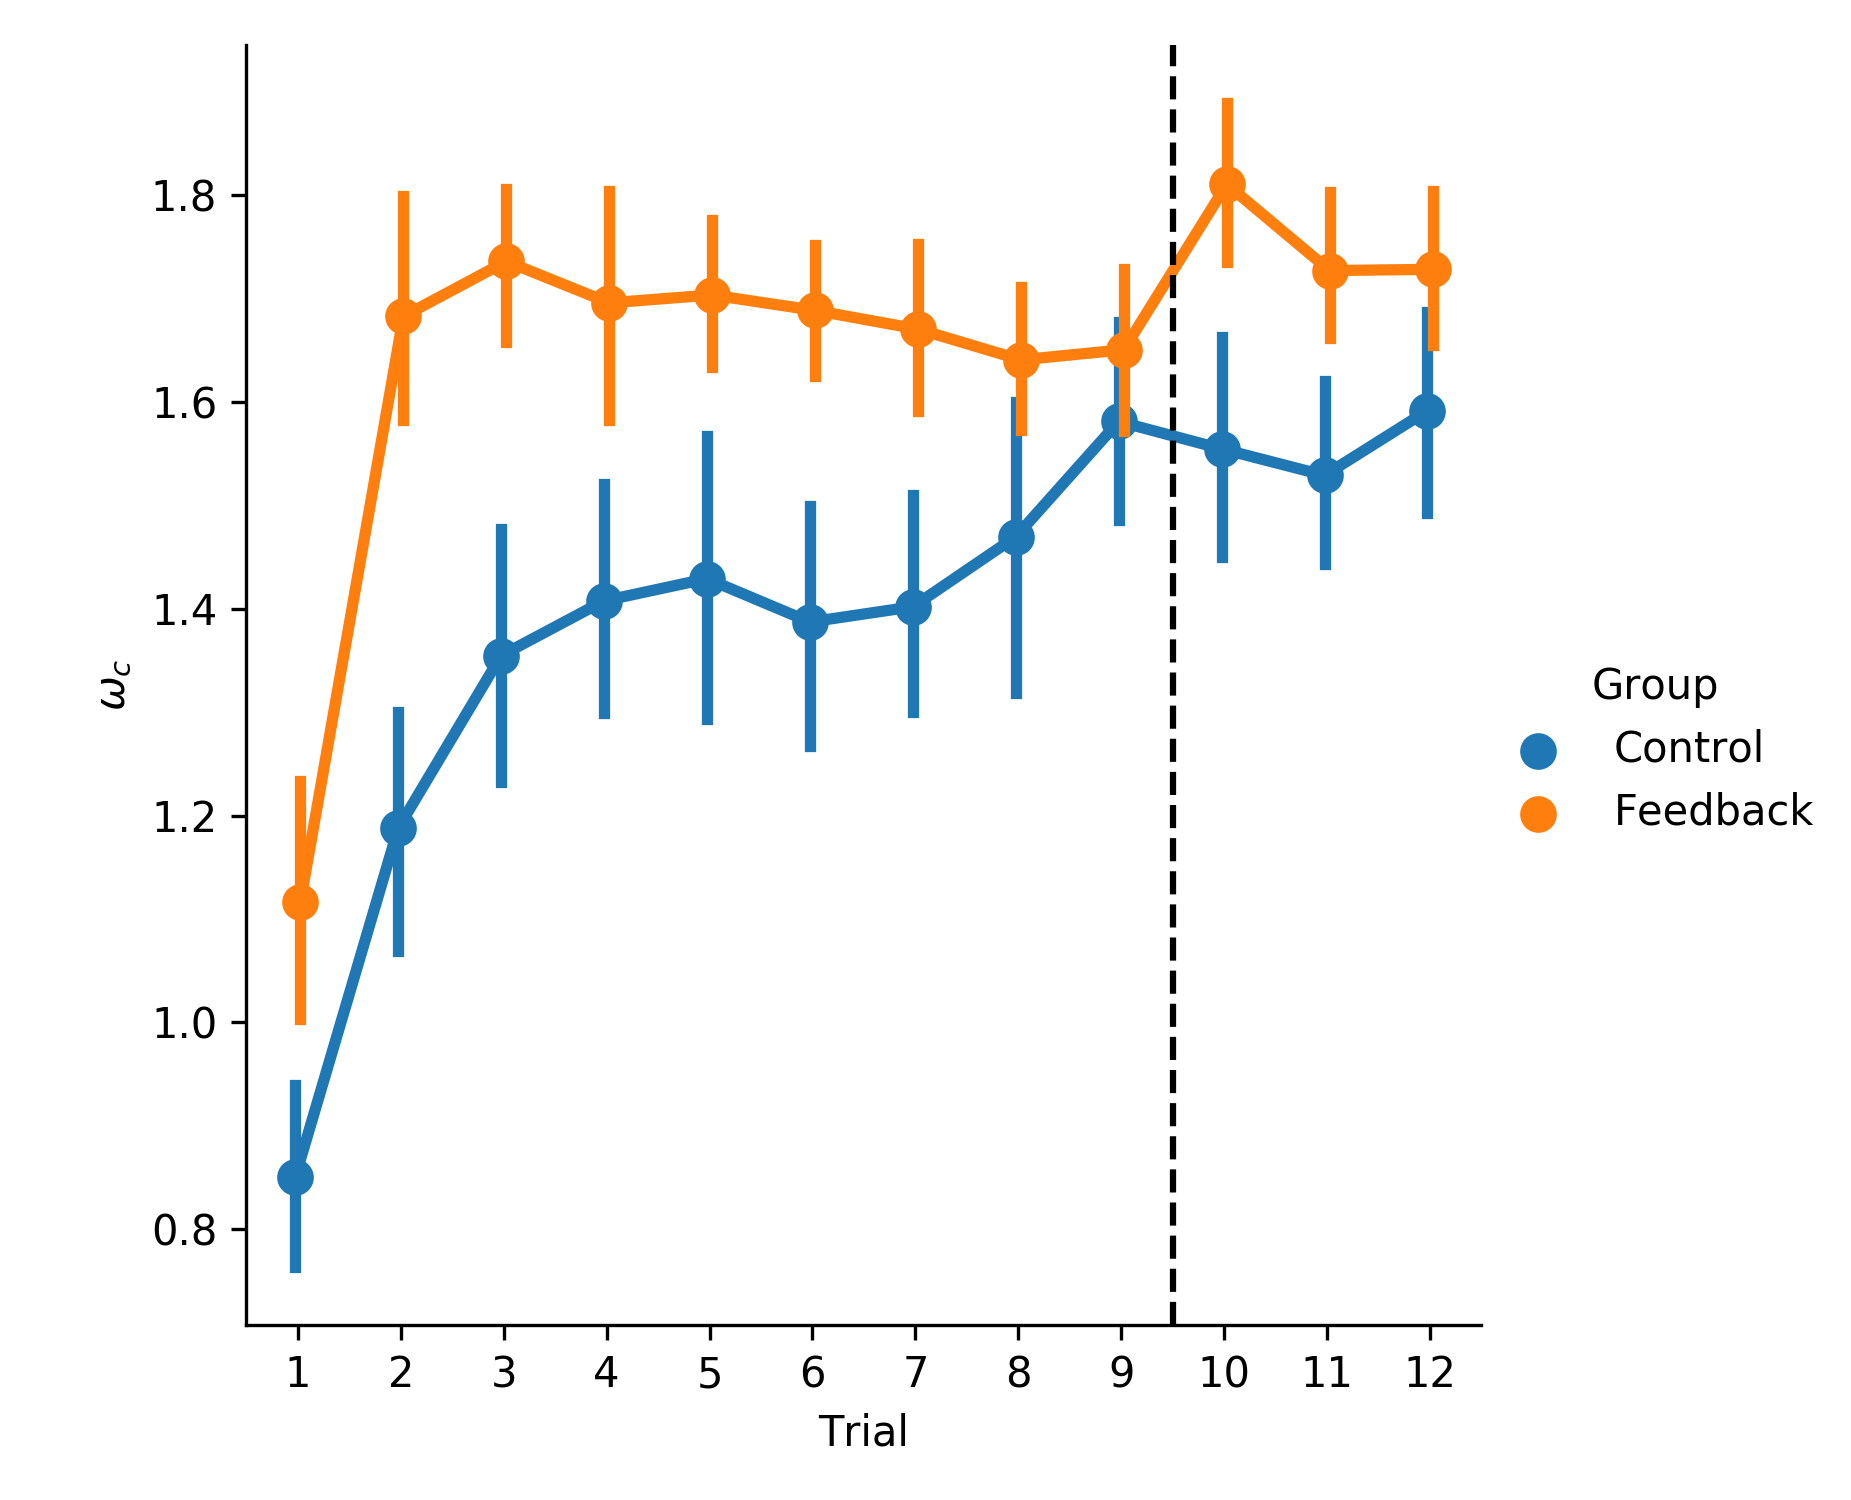
\includegraphics[width=0.8\linewidth]{figures/Modeling/wc_arx.png}
    \caption[Crossover frequency (ARX)]{Crossover frequency predicted by the ARX technique for the pitch only trials.}
    \label{fig:arx_crossover}
\end{figure}

Mixed models were used to calculate the significance of factors in our analysis due to the presence of performance outliers which were removed from the analysis.
The Satterthwaite method was used to calculate the adjusted degrees of freedom using the lmerTest package in R~\citep{RN53}.
When significant effects were observed, post hoc comparisons using the Tukey Honest Significance Difference (HSD) test were performed and considered significant at the $p < .05$ level, and the Satterthwaite method was again used to calculate the degrees of freedom.
Only 7 of the 1080 total trials (30 subjects with 36 trials per subject) were removed.
These trials were extreme performance outliers and including these trials does not change the primary results of the study.

A three-factor (Group, Mode, and Trial) mixed model with two repeated measures (Mode and Trial) was run on the pitch crossover frequency.
There were significant main factors of group $(F(1, 28.00) = 4.9, p = 0.036)$, mode $(F(2, 55.62) = 17.1, p < .001)$, and trial $(F(11, 306.23) = 39.4, p < .001)$.
There were also significant interaction effects between group and trial $(F(11, 306.23) = 2.0, p = 0.025)$ and between mode and trial $(F(22, 610.08) = 2.8, p < .001)$.
Despite the presence of interaction effects that result from participants learning the task (as indicated by the trial factor), the main effects can still be interpreted.
A Tukey test showed that the participants in the groups differed significantly, with the participants in the feedback group outperforming those in the control group $(M = 1.25, 1.56,$ respectively, $SE = 0.10)$.
An additional Tukey test showed that the participants' crossover frequency between the modes differed significantly, with the largest crossover frequency in the P mode, followed by the PR mode, and finally the lowest in the PRA mode $(M = 1.53, 1.38, 1.31$ respectively, $SE = 0.07)$.
This same analysis was completed on the roll crossover frequency, with similar results.
There were significant main factors of group $(F(1, 27.82) = 8.2, p < 0.01)$, mode $(F(1, 25.49) = 23.2, p < 0.001)$, and trial $(F(11, 292.40) = 16.3, p < .001)$.
Tukey tests showed that the participants' crossover frequency between the groups and the modes each differed significantly, with the participants in the feedback group again outperforming those in the control group $(M = 0.55, 0.89,$ respectively, $SE = 0.08)$, and crossover frequency was best in the PR mode followed by the PRA mode $(M = 0.77, 0.67,$ respectively, $SE = 0.06)$.
A two-factor (Group and Trial) mixed model with one repeated measure (Trial) was run on the altitude crossover frequency.
There were significant main factors of group $(F(1, 27.92) = 4.4, p = 0.046)$ and trial $(F(11, 301.95) = 18.3, p < .001)$.
Tukey tests showed that the participants' crossover frequency between the groups differed significantly, with the participants in the feedback group again outperforming those in the control group $(M = 0.98, 1.29,$ respectively, $SE = 0.11)$, and the trial effect showing learning throughout the experiment for both groups.
See Figure~\ref{figure:arxcomplete} for the plots of the crossover frequency of the estimated pilot/vehicle open-loop transfer functions for each group, trial, and control task.

\begin{figure}[tb]
    \begin{center}
        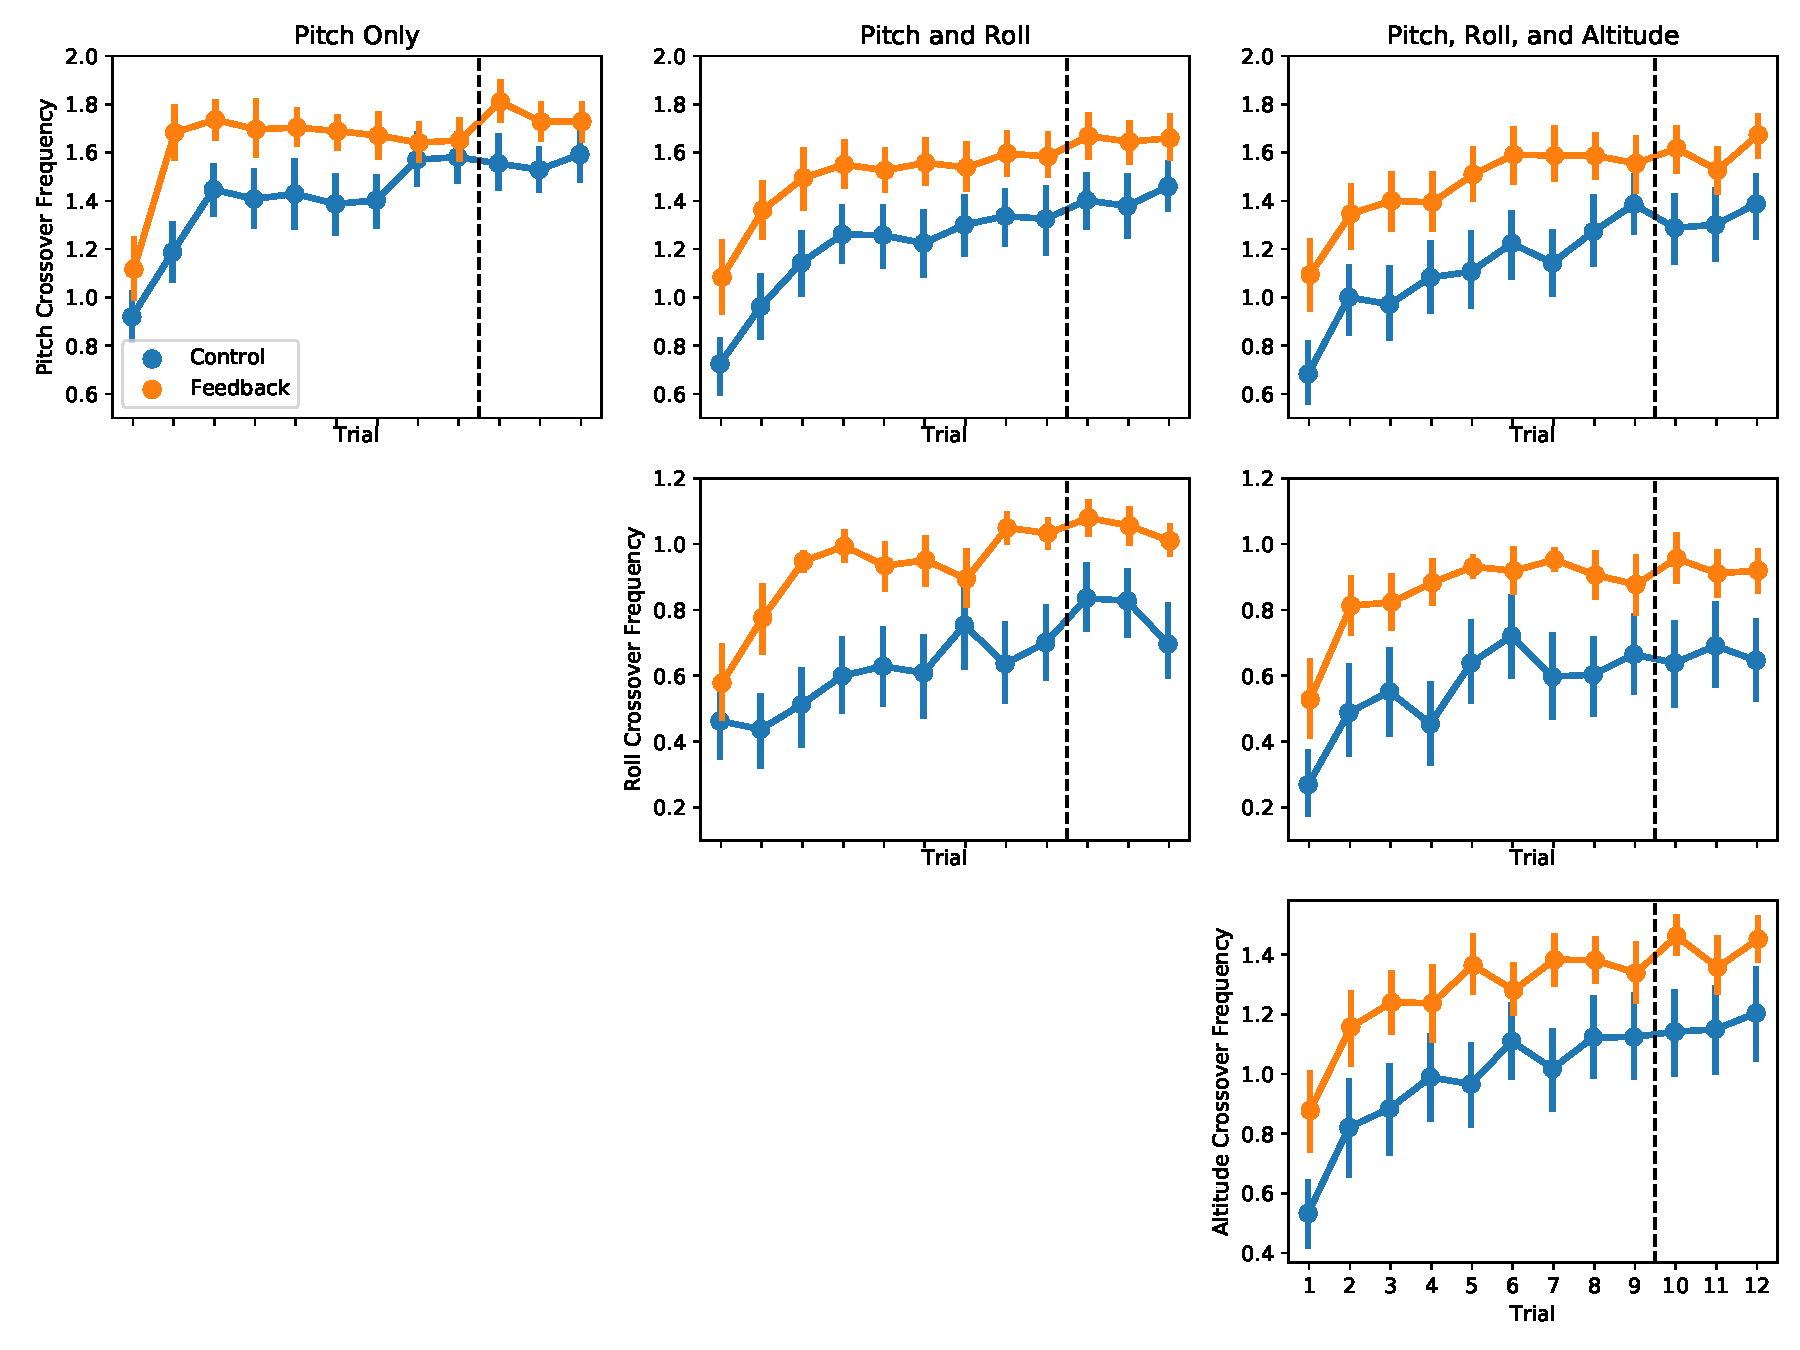
\includegraphics[width=\linewidth]{figures/Modeling/crossover_measures.pdf}
        \caption[The crossover frequency of the estimated pilot/vehicle open-loop transfer functions for each group, trial, and control task]{The crossover frequency of the estimated pilot/vehicle open-loop transfer functions for each group, trial, and control task.
                The dashed line indicates where the feedback was removed from participants in the feedback group.
                Error bars are the standard error of the mean.}
        \label{figure:arxcomplete}
    \end{center}
\end{figure}

\subsection{Structural Model}
\subsubsection{Value Identification Technique}
Once the Structural Model was parameterized to the version presented in Figure~\ref{fig:structuralmodelreduced}, the problem then becomes best fitting the remaining parameters to best match the data collected in the experiment.
This is more complicated than the ARX technique as there are many parameters to identify which interact nonlinearly, and the fit function has many local maximums.

A four-step process was developed to tackle the problem of finding the optimal model parameters, the results of which were compared to the results of the ARX technique to validate our approach.
The general outline of the technique was:
\begin{enumerate}
    \item Conduct a brute force parameter search over the six remaining model parameters.
    \item Identify the set of parameters that results in a maximum VAF as an initial best guess.
    \item Iterate on the initial guess to identify a final optimal set of parameters.
    \item Identify the crossover frequency using the system dynamics and identified optimal parameters.
\end{enumerate}
Each of these steps is further described below.

\begin{table}[tb]
    \centering
    \includetable{modeling-structural-model-parameters.tex}
    \caption[Structural Model parameters used for the initial global optimal fit]{Structural Model parameters used for the initial global optimal fit.}
    \label{table:structuralmodelparameters}
\end{table}

The first step of the value identification technique was a brute force parameter search used to identify the value of the remaining parameters.
Each combination of the parameters $K_e, \tau_0, K, a$, $\omega_{NM}$ and $\zeta_{NM}$ were enumerated over and simulated in Simulink using the same flight model and disturbance profiles as the participants experienced in the experiment, see Table~\ref{table:structuralmodelparameters}.
The values from this table were chosen based on a coarse preliminary analysis such that they covered the expected range of values with sufficient granularity.
The resulting 102,600 simulations were compared to each trial to identify the set of parameter values resulting in the smallest VAF.
Each combination of experimental subject data and simulations was then compared to find a set of simulation parameters that maximized the VAF.
This solution represented a globally maximum set of a parameters, mitigating the issue resulting from the parameters nonlinear interaction with each other.
Once this initial global best fit was identified, the parameters were further tuned in MATLAB using ``fmincon'' to find the minimum of the constrained nonlinear multivariable function, which was the maximum VAF.
The constraints for the solver were the bounds of the global brute force search, though, in general, the optimizer did not result in large parameter changes from the initial values.
An interaction effect between trying to simultaneously fit $\omega_{NM}$ and $\zeta_{NM}$ initially resulted in convergence issues.
To resolve this issue, $\zeta_{NM}$ was left out of the initial optimization step and tuned independently at the end of the optimization process.
Finally, the the identified set of six parameters was inserted into the model and combined with the controlled system dynamics to identify the resultant crossover frequency.
The resulting crossover frequency of this technique (Figure~\ref{fig:sm_crossover}) compares very favorably with that found using the ARX technique (Figure~\ref{fig:arx_crossover}).
Both techniques show an initially small crossover frequency which approaches the generally accepted upper limit of $\approx 1.7-2$ rad/s~\citep{hess1984analysis}.

\begin{figure}[tb]
    \centering
    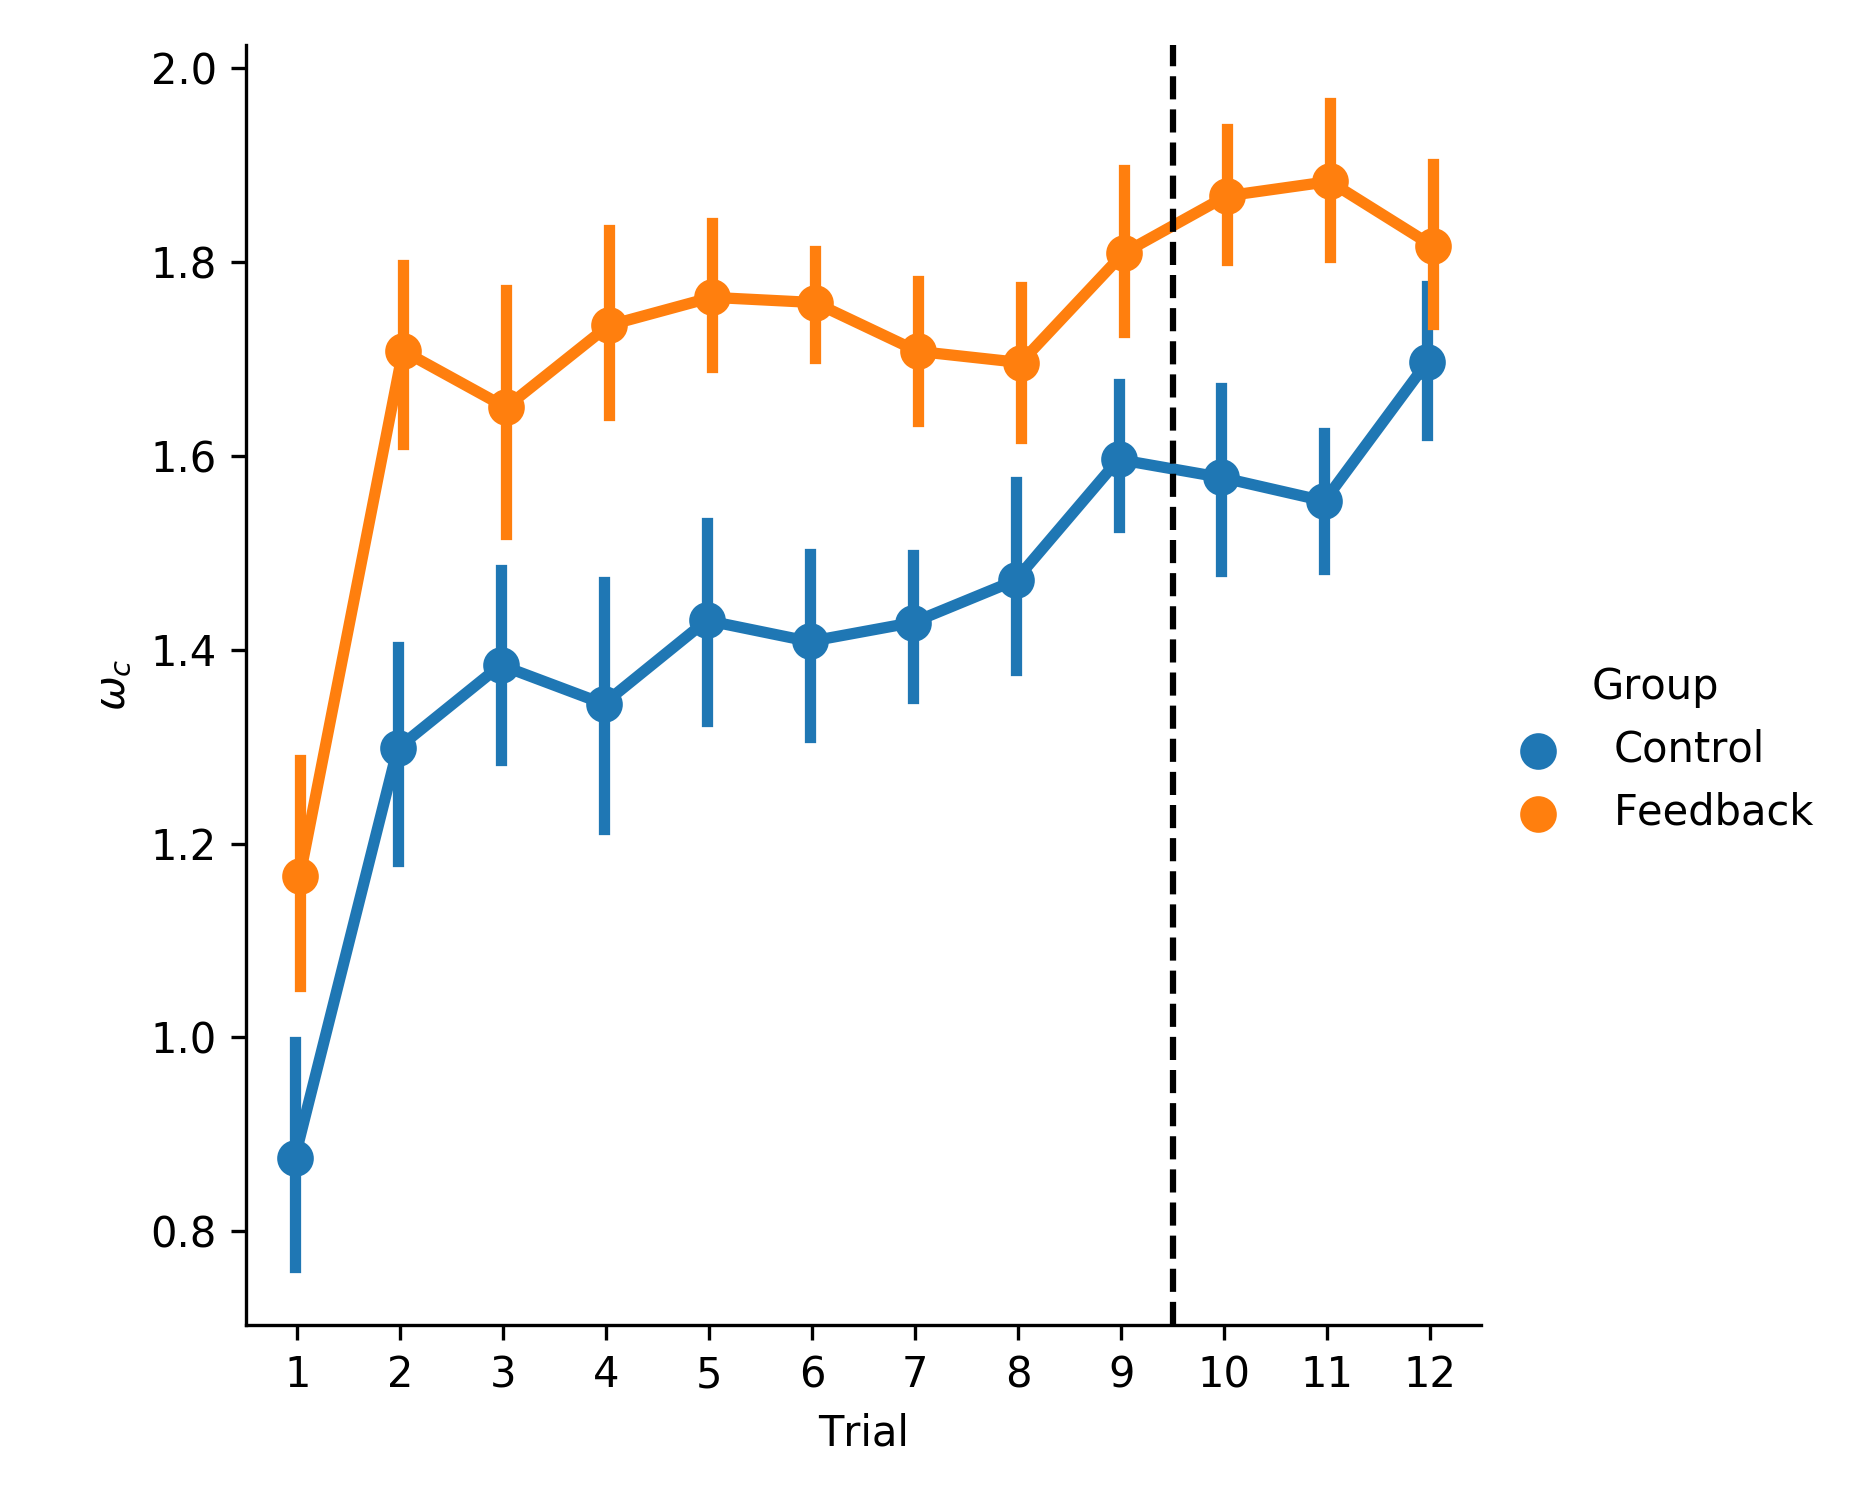
\includegraphics[width=0.8\linewidth]{figures/Modeling/wc_group.png}
    \caption[Crossover frequency (Structural Model)]{Crossover frequency predicted by the Structural Model parameter identification for the pitch only trials.}
    \label{fig:sm_crossover}
\end{figure}

Only the first control mode, Pitch only, was analyzed for the results presented below.
The technique developed here could be extended to all three control loops however, and the results should be similar (and more pronounced for modes of higher complexity).
By investigating the control mode with the smallest effect of the feedback, we show that this technique is sensitive enough to detect small changes between the two groups.
A two-factor (Group and Trial) mixed model with repeated measures (Trial) was run on each of the six parameters to identify which parameters significantly changed between groups and over the course of training.
As with the ARX technique, the Satterthwaite method was used to calculate the adjusted degrees of freedom.
The results of this analysis are presented in Table~\ref{table:structuralmodelmixed}.

\begin{table}[tb]
    \centering
    \includetable{modeling-structural-model-mixed.tex}
    \caption[Results of the linear mixed models of the identified Structural Model parameters]{Results of the linear mixed models of the identified Structural Model parameters.}
    \label{table:structuralmodelmixed}
\end{table}

Evaluating the results of the linear mixed effects models presented in Table~\ref{table:structuralmodelmixed}, we immediately see that $\tau_0, K,$ and $\omega_{NM}$ have no significant effects dividing either Group or Trial.
From this we can determine that these variables have no significant effect resulting from either training or the difference in performance between the feedback and control groups.
Of the remaining variables, $a$ and $\zeta_{NM}$ show significant effects in the trial factor, suggesting that the change with time.
Further investigation on these variables showed that $a$ was only significantly different for the very first trial, a result which was ignored for the remainder of this analysis to simplify the resulting model.
$\zeta_{NM}$ also varied significantly as a result of training, but further investigating showed that the effects of varying this parameter did not significantly affect the resulting outputs of the model.
As a result of this, $\zeta_{NM}$ was not considered an important variable to include in the feedback model.
Finally, the $K_e$ variable showed significant effects between both the Group and Trial variables, suggesting that it was the primary parameter responsible for changes in performance between the groups and as a result of repeated training in the simulator.
As a consequence of this result, modifying this parameter to explain the results of increased performance in the feedback group became the focus of the remainder of this chapter.

\section{Extending the Structural Model}
\begin{figure}[tb]
    \centering
    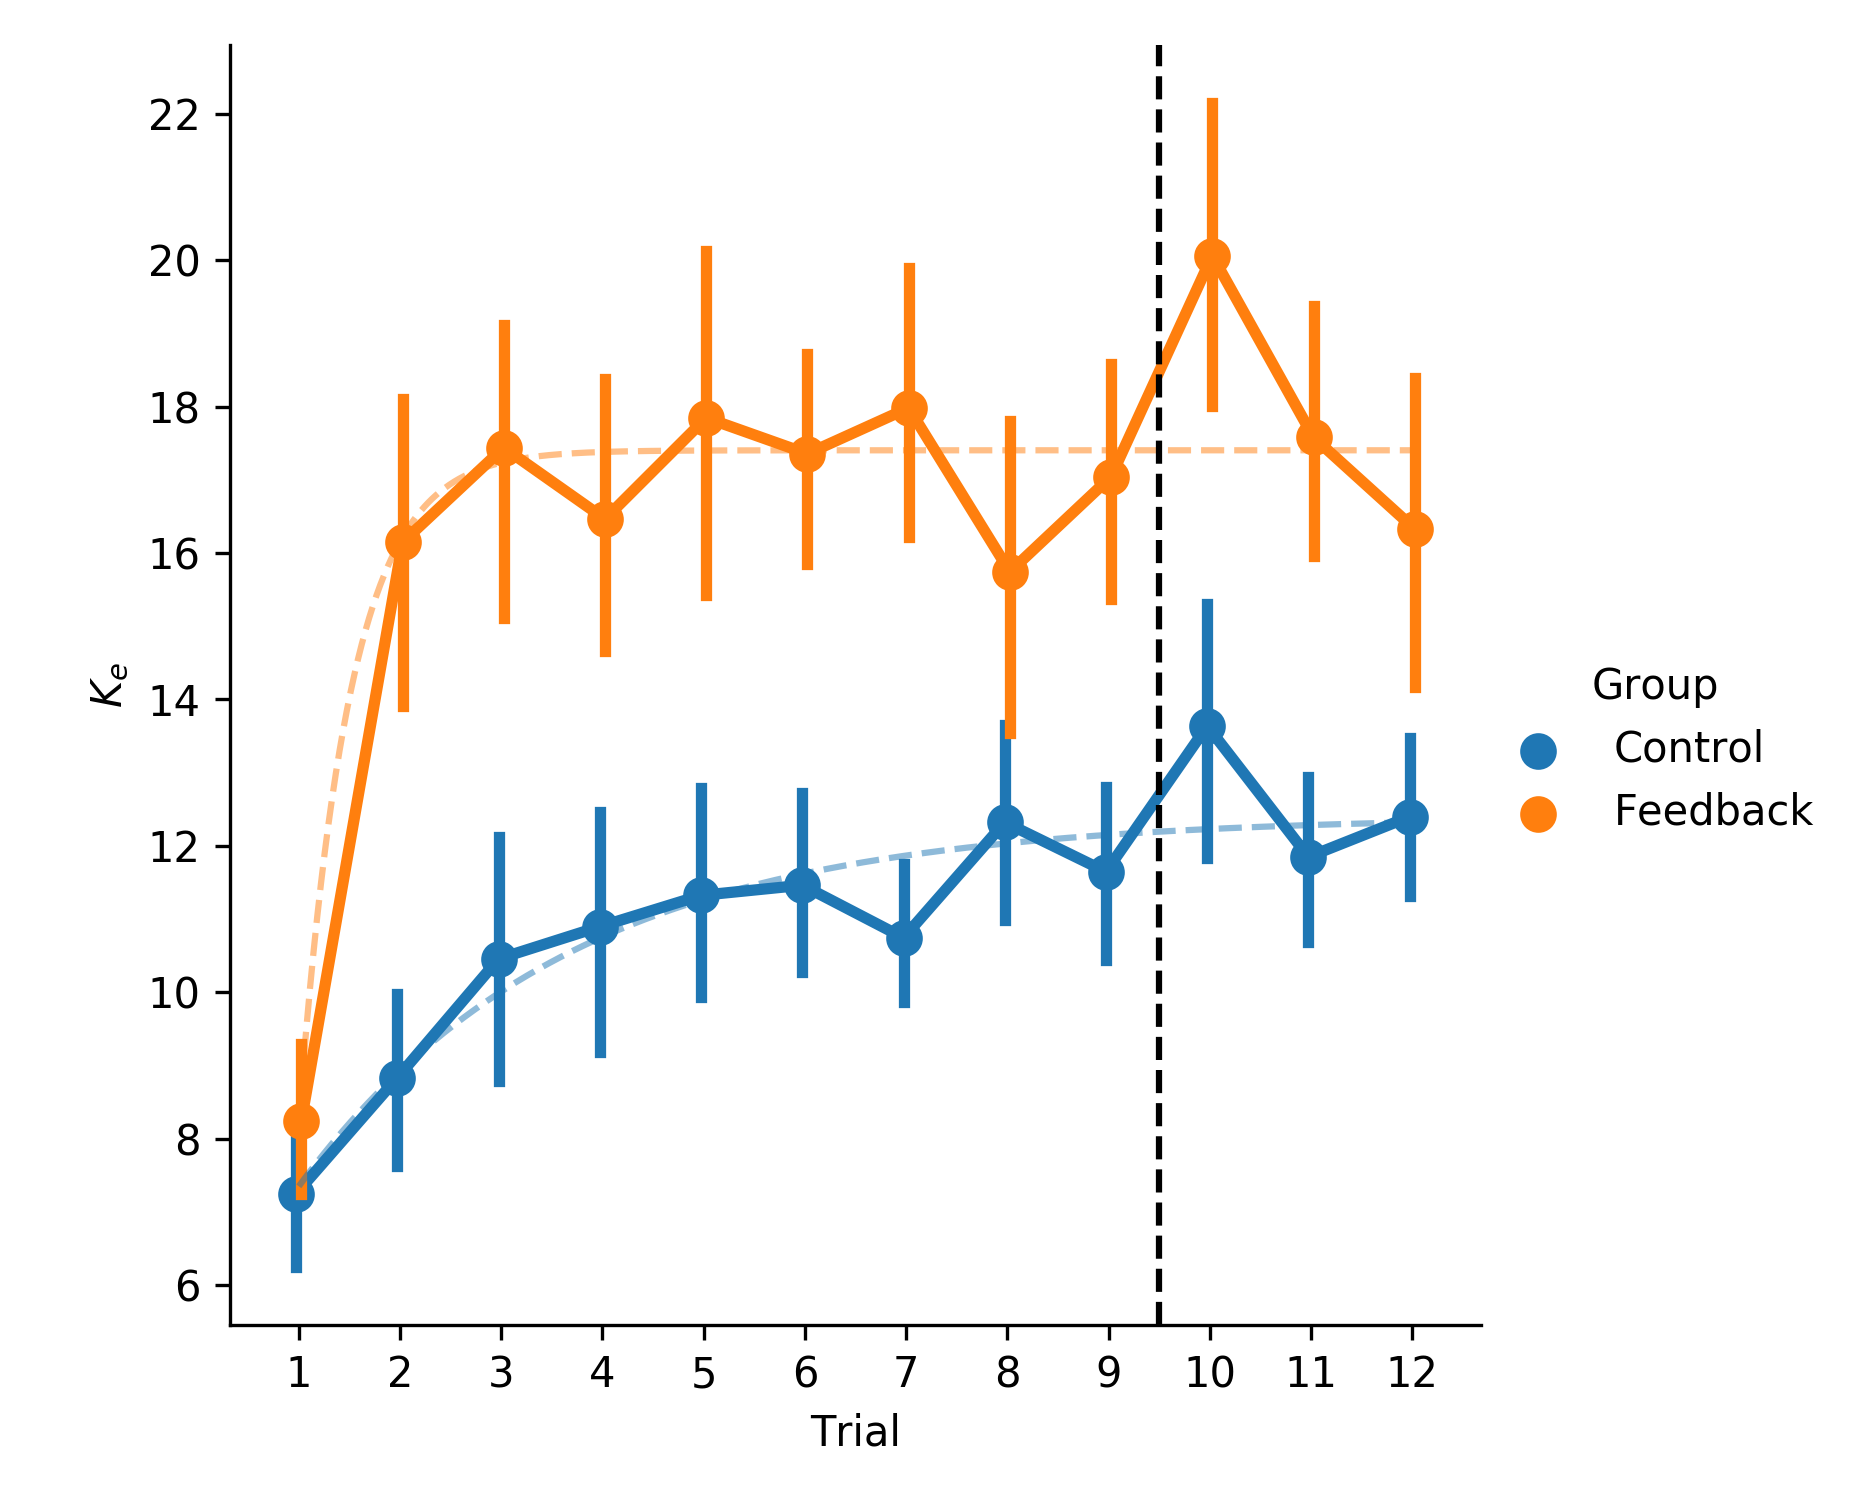
\includegraphics[width=0.8\linewidth]{figures/Modeling/ke_group.png}
    \caption[$K_e$ is greater for subjects exposed to feedback]{$K_e$ is greater for subjects exposed to feedback.}
    \label{fig:ke_group}
\end{figure}

As a result of the analysis resulting from the linear mixed effects models, we determined that all the parameters can be treated as constants with the exception of $K_e$, which changes with both Trial and Group.
The resulting values for the remainder of the parameters were averaged and identified as the values listed in Table~\ref{table:structuralmodelresultants}, see below.
\begin{table}[tb]
    \centering
    \includetable{modeling-structural-model-resultants.tex}
    \caption[Identified optimal parameters of the Structural Model for the Aircraft Flight Task]{Identified optimal parameters of the Structural Model for the Aircraft Flight Task.}
    \label{table:structuralmodelresultants}
\end{table}
Note that the standard error of the mean for the identified values was quite low, further reinforcing how little they changed between subjects, trials, and group.
The final parameter, $K_e$, can be modeled as an exponential function that increases with training, see Figure~\ref{fig:ke_group}.
$K_e$ was modeled for each group as a function of trial with three parameters, such that
\begin{align} \label{eq:kefit}
    K_e = A e^{(-B*\mbox{Trial})}+C
\end{align}
where $A$ is the scale factor, $B$ describes how rapidly $K_e$ changes with trial, and $C$ is a baseline value.
The results of least squares best fits to the data are presented in Table~\ref{table:kevalues}.
\begin{table}[tb]
    \centering
    \includetable{modeling-structural-ke-values.tex}
    \caption[Identified $K_e$ parameters for the two groups]{Identified $K_e$ parameters from Equation~\ref{eq:kefit} for the two groups.}
    \label{table:kevalues}
\end{table}
The resulting fit well represents the values identified by the value identification technique, and reflects what we have observed throughout this analysis--that the feedback group learns much more quickly and results in better performance (and a large $K_e$) than the control group.

We propose that the $K_f$, the change between the identified $K_e$ of the control and feedback groups, determines the change in performance of subjects exposed to the feedback.
We further propose that this $K_f$ is a result of the accumulation of exposure to feedback, such that
\begin{align}
    K_f       & = K_{eF} - K_{eC}                  \\
    K_f       & \propto \int \mbox{Feedback}(t) dt \\
    \dot{K_f} & \propto \mbox{Feedback}(t)
\end{align}
where $K_{eC}$ and $K_{eF}$ are the $K_e$ variables identified from exponential fits to the $K_e$ variable for the control and feedback groups, respectively.
Here we have defined $K_f$ as a variable proportional to the total accumulated time operators were exposed to the feedback, and $\dot{K_f}$ is defined as change in $K_f$ trial-to-trial which results from the time exposed to the feedback in a given trial.

\begin{figure}[tb]
    \centering
    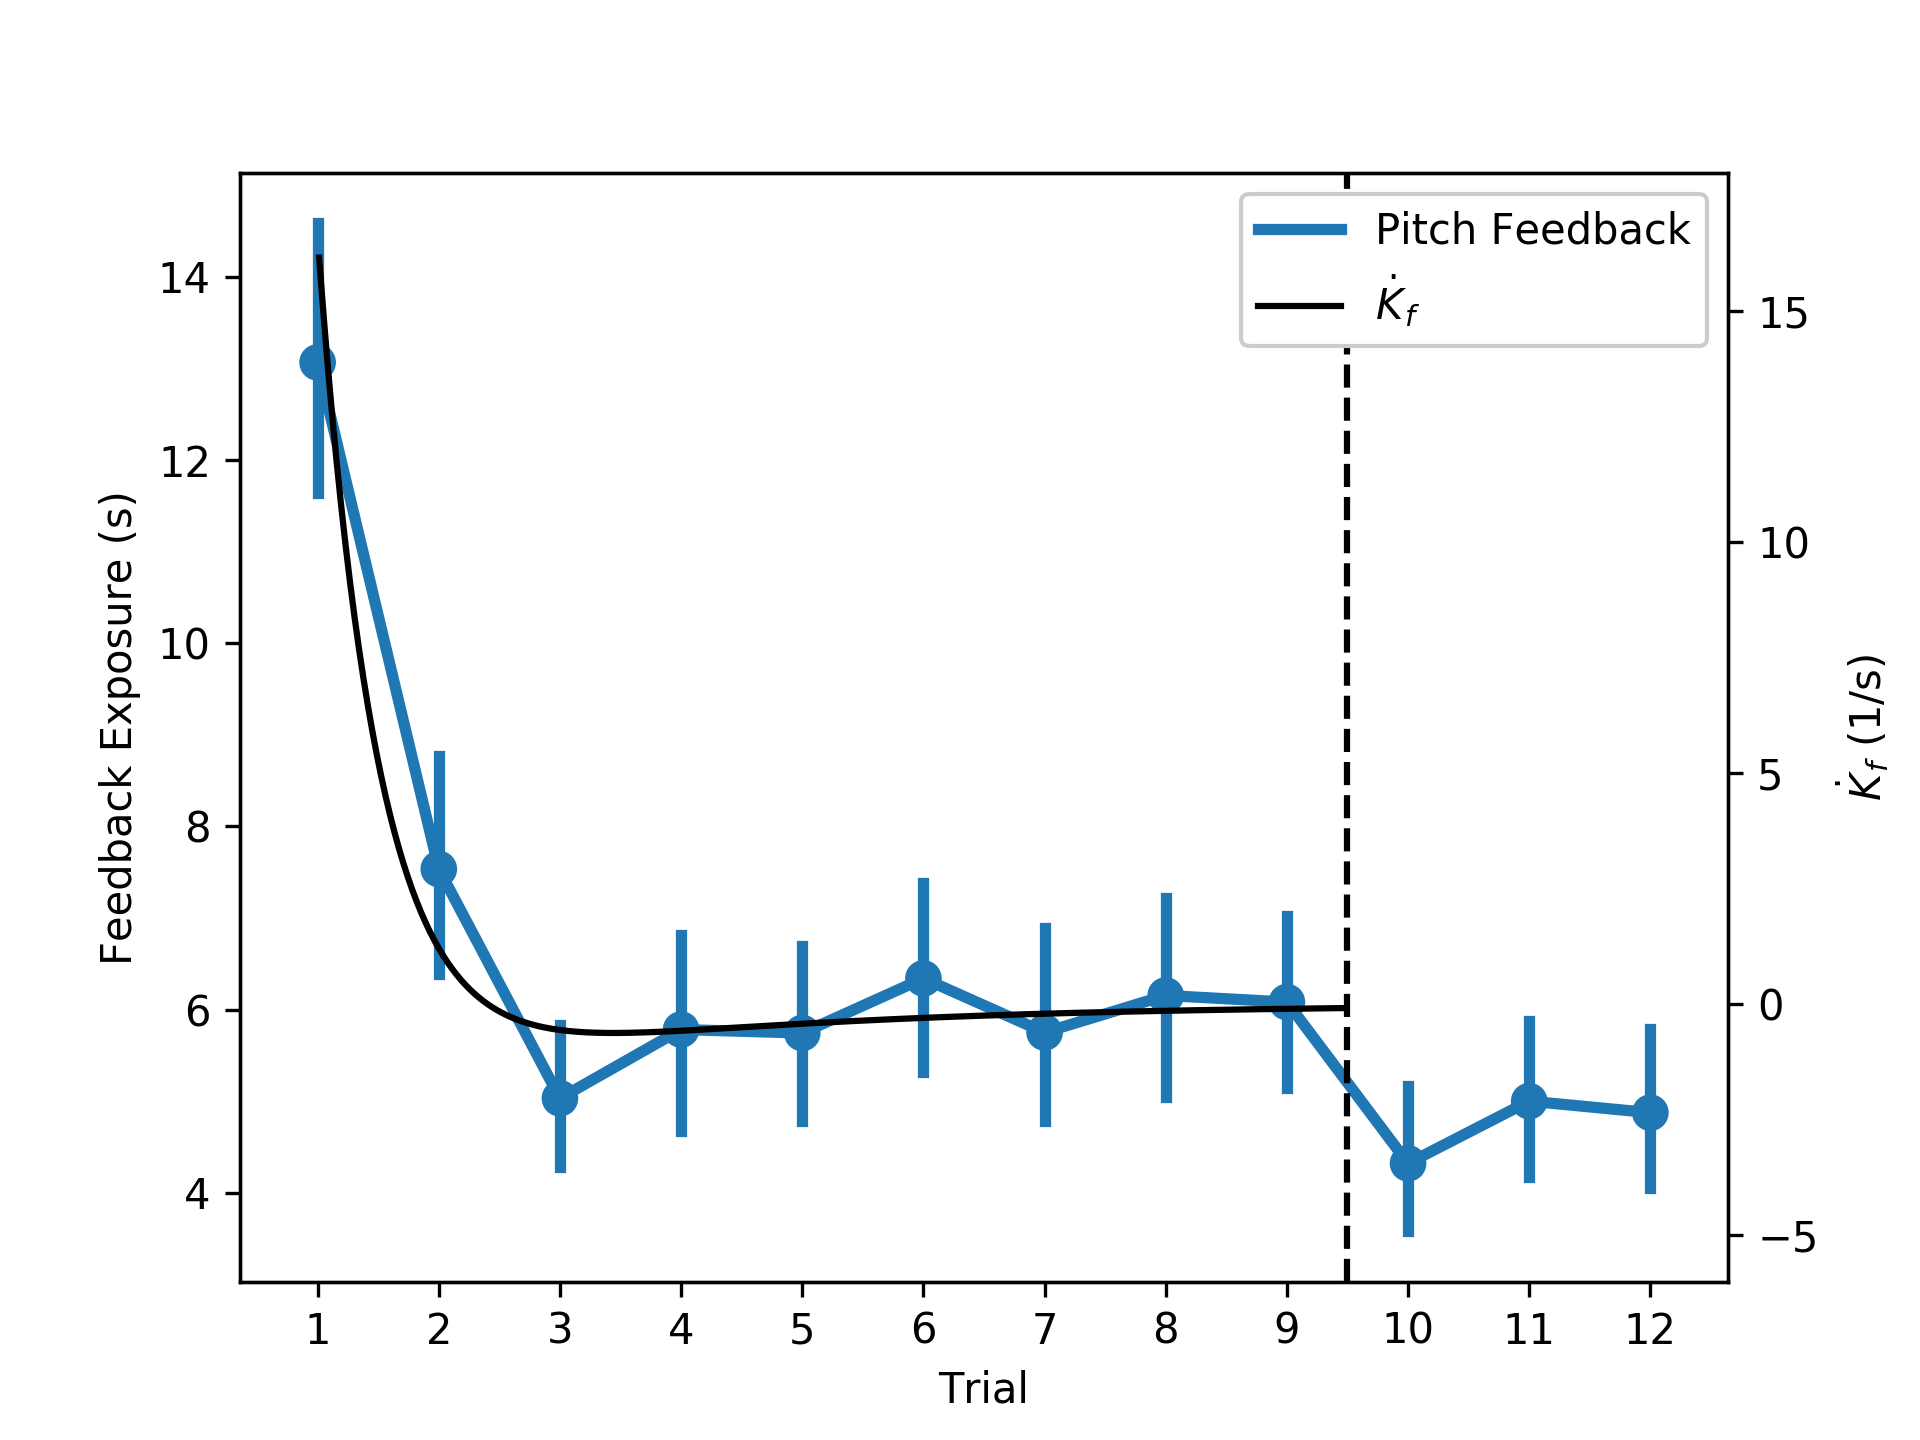
\includegraphics[width=0.8\linewidth]{figures/Modeling/f_v_kfd.png}
    \caption[The feedback exposure time directly correlates with $\dot{K_{f}}$]{The feedback exposure time directly correlates with $\dot{K_{f}}$ which confirms that the accumulation of exposure to feedback drives $K_f$.}
    \label{fig:feedback_kfd}
\end{figure}

We can test this proposal by plotting average time subjects in the feedback group were exposed to the feedback in each trial and comparing this to the value of $\dot{K_f}$ calculated from the derivative of the exponential fits.
This comparison is available in Figure~\ref{fig:feedback_kfd}.
Here we see that the data from the experiment is directly proportional to the modeled value $\dot{K_f}$, suggesting that our proposal is a viable explanation of the observed effects.
$\dot{K_f}$, which can also be thought of as the change in the amount benefit that subjects in the feedback group have over the control group in a given trial, sharply decreases over the first few trials to a steady value.
This confirms what we observed in the experiment--that subjects gain most of the benefit from feedback very quickly, in just a few trials.
Further analysis of Figure~\ref{fig:feedback_kfd} shows that, for this task, an exposure period of approximately 6 seconds (or $6/82\approx0.07\%$) in a trial leads to no change in performance.
At this time, it is unclear if this amount or percentage of time is task dependent, or if, for example, it simply represents the average boundary of human control for this task.
As a result of this analysis, the proposed modified version of the Structural Model is available in Figure~\ref{fig:structuralmodel_feedback}.

\begin{figure}[tb]
    \centering
    \includegraphics[width=0.8\linewidth]{figures/structural_model_reduced_modified/structural_model.pdf}
    \caption[The proposed addition to the Structural Model to account for concurrent bandwidth feedback]{The proposed addition to the Structural Model to account for concurrent bandwidth feedback (CBF).}
    \label{fig:structuralmodel_feedback}
\end{figure}

\section{Discussion}
We were interested in using a pilot modeling approach to explain the differences in performance that we observed from the aircraft flight task study explored in Chapter~\ref{chapter:aircraftfeedback}).
In this study, subjects repeatedly trained on flight tasks of increasing functional complexity, and one group of subjects received visual concurrent bandwidth feedback.
We explored two different modeling strategies, an ARX based technique called \textit(gettf1) and the Hess Structural Model.

A time-domain autoregressive exogenous (ARX) identification technique was used to estimate pilot transfer functions.
The estimated combined pilot/vehicle open-loop transfer functions were evaluated to determine the evolution of the crossover frequency for each control loop throughout training.
Results indicate that participants in the feedback group had a significantly lower root-mean-square error and higher crossover frequency than those in the control group, indicating better performance.
The ARX identification technique provided a consistently high variance accounted for (VAF), indicating that it can identify transfer functions representing a variety of operators at various levels of training.
These results are more pronounced for modes with increased functional complexity and persisted in retention testing when the feedback was removed, indicating that participants were not reliant on the feedback.

The Hess Structural Model of the pilot was also investigated, which ``describe[s] the underlying structure which contributes to human pilot dynamics.''
The Structural Model is of interest for interpreting the effects of concurrent feedback as it incorporates multiple sensory channels and models of visual acuity and the time-varying human pilot.
We developed a novel approach for identifying the parameters in the Structural Model from experimental subject data.
This approach was validated by comparing the crossover frequency identified from the ARX technique, which showed that both techniques identified a similar evolution of the crossover frequency with training and between groups.
The result of a linear mixed effects model showed that, of the six parameters which were fit, only $K_e$, the leading visual gain, varied between both group and trial.

An extension to the Structural Model was proposed which explains the effects observed when operators are exposed to concurrent bandwidth feedback.
This proposed model includes the addition of a single additional parameter, $K_f$, which accumulates when the operator is exposed to feedback.
This parameter is added in the primary control loop, next to the $K_e$ term, and results in operators performing the task with a statistically lower root-mean-square error.
This exposed to the feedback also immediately approach the limit of human control, with identified crossover frequency values of $\approx 1.7-2$ rad/s.
